\section{Poisson distribution}

\begin{table}[H]
    \hfill
    \begin{minipage}{0.45\linewidth}
        \begin{figure}[H]
            \centering
            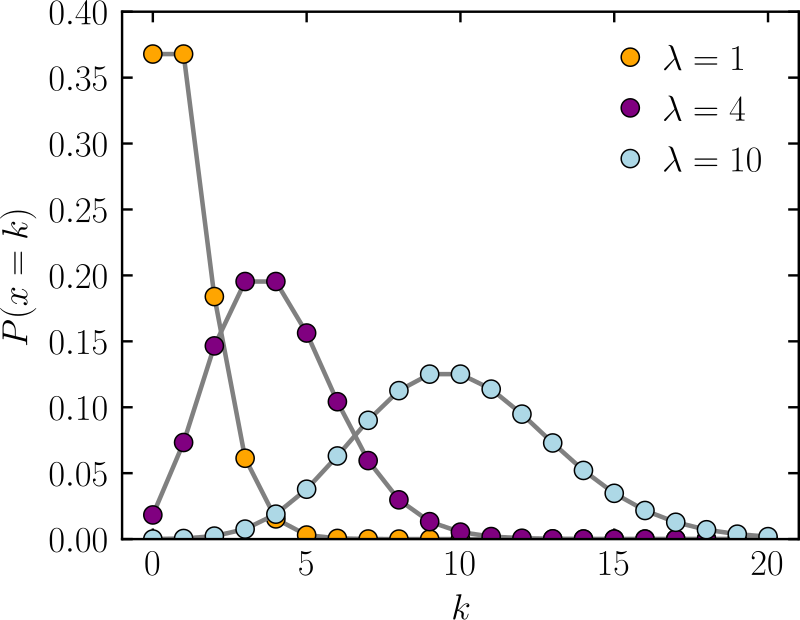
\includegraphics[
                width=\linewidth,
                height=5cm,
                keepaspectratio,
            ]{images/distributions/Poisson_pmf.svg.png}
            \caption{Poisson distribution: PDF \cite{wiki/Poisson_distribution}}
        \end{figure}
    \end{minipage}
    \hfill
    \begin{minipage}{0.45\linewidth}
        \begin{figure}[H]
            \centering
            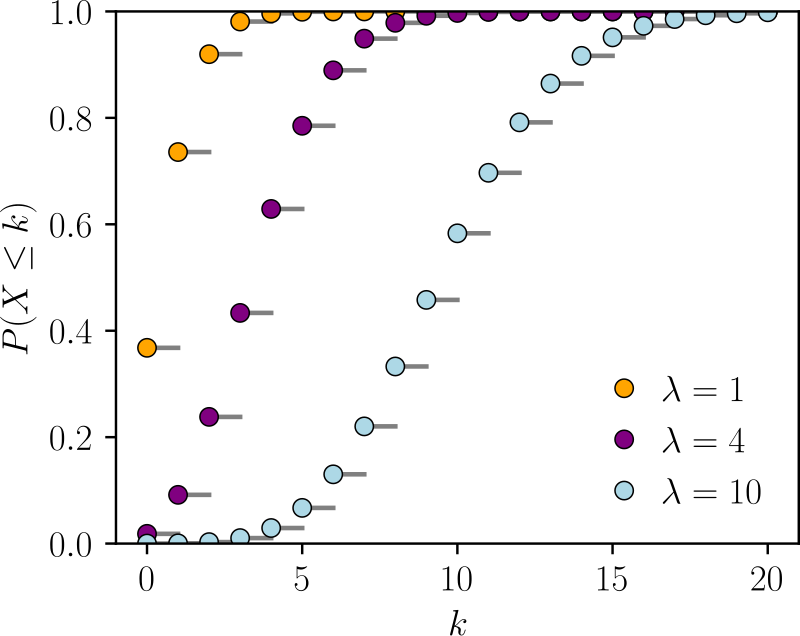
\includegraphics[
                width=\linewidth,
                height=5cm,
                keepaspectratio,
            ]{images/distributions/Poisson_cdf.svg.png}
            \caption{Poisson distribution: CDF \cite{wiki/Poisson_distribution}}
        \end{figure}
    \end{minipage}
    \hfill
\end{table}







\subsection{Summary}

\begin{enumerate}
    \item \textbf{Notation}: 
    $
         {\displaystyle \operatorname {Pois} (\lambda )}
    $
    \hfill \cite{wiki/Poisson_distribution}

    \item \textbf{Parameters}:
    ${\displaystyle \lambda \in (0,\infty )}$ (rate)
    \hfill \cite{wiki/Poisson_distribution}

    \item \textbf{Support}: 
    ${\displaystyle k\in \mathbb {N} _{0}}$ (Natural numbers starting from $0$)
    \hfill \cite{wiki/Poisson_distribution}

    \item \textbf{PMF}:
    $ 
         {\displaystyle {\frac {\lambda ^{k}e^{-\lambda }}{k!}}}
    $
    \hfill \cite{wiki/Poisson_distribution}

    \item \textbf{CDF}:
    ${\displaystyle {\frac {\Gamma (\lfloor k+1\rfloor ,\lambda )}{\lfloor k\rfloor !}},}$ or
    ${\displaystyle e^{-\lambda }\sum _{j=0}^{\lfloor k\rfloor }{\frac {\lambda ^{j}}{j!}},}$ or
    ${\displaystyle Q(\lfloor k+1\rfloor ,\lambda )}$
    (for ${\displaystyle k\geq 0,}$ where ${\displaystyle \Gamma (x,y)}$ is the upper incomplete gamma function, ${\displaystyle \lfloor k\rfloor }$ is the floor function, and ${\displaystyle Q}$ is the regularized gamma function)
    \hfill \cite{wiki/Poisson_distribution}

    \item \textbf{Mean}: 
    $ 
         {\displaystyle \lambda }
    $
    \hfill \cite{wiki/Poisson_distribution}

    \item \textbf{Median}: 
    $
         {\displaystyle \approx \left\lfloor \lambda +{\frac {1}{3}}-{\frac {1}{50\lambda }}\right\rfloor }
    $
    \hfill \cite{wiki/Poisson_distribution}

    \item \textbf{Mode}: 
    $
         {\displaystyle \left\lceil \lambda \right\rceil -1,\left\lfloor \lambda \right\rfloor }
    $
    \hfill \cite{wiki/Poisson_distribution}

    \item \textbf{Variance}: 
    $ 
         {\displaystyle \lambda }
    $
    \hfill \cite{wiki/Poisson_distribution}

    % \item \textbf{Median absolute deviation (MAD)}: 
    % $    
    % $
    % \hfill \cite{wiki/Poisson_distribution}

    \item \textbf{Skewness}:
    $
         {\displaystyle {\frac {1}{\sqrt {\lambda }}}}
    $
    \hfill \cite{wiki/Poisson_distribution}

    \item \textbf{Excess kurtosis}: 
    $
         {\displaystyle {\frac {1}{\lambda }}}
    $
    \hfill \cite{wiki/Poisson_distribution}

    \item \textbf{Entropy}: 
    ${\displaystyle \lambda {\Bigl [}1-\log(\lambda ){\Bigr ]}+e^{-\lambda }\sum _{k=0}^{\infty }{\frac {\lambda ^{k}\log(k!)}{k!}}}$ 
    or for large ${\displaystyle \lambda }$
    ${\displaystyle {\begin{aligned}\approx {\frac {1}{2}}\log \left(2\pi e\lambda \right)-{\frac {1}{12\lambda }}-{\frac {1}{24\lambda ^{2}}}\\-{\frac {19}{360\lambda ^{3}}}+{\mathcal {O}}\left({\frac {1}{\lambda ^{4}}}\right)\end{aligned}}}$
    \hfill \cite{wiki/Poisson_distribution}

    \item \textbf{Moment-generating function (MGF)}: 
    $
         {\displaystyle \exp \left[\lambda \left(e^{t}-1\right)\right]}
    $
    \hfill \cite{wiki/Poisson_distribution}
    
    \item \textbf{Characteristic function (CF)}:
    $   
         {\displaystyle \exp \left[\lambda \left(e^{it}-1\right)\right]}
    $
    \hfill \cite{wiki/Poisson_distribution}

    \item \textbf{Probability-generating function (PGF)}:
    $
         {\displaystyle \exp \left[\lambda \left(z-1\right)\right]}
    $
    \hfill \cite{wiki/Poisson_distribution}

    \item \textbf{Fisher information}:
    $
         {\displaystyle {\frac {1}{\lambda }}}
    $
    \hfill \cite{wiki/Poisson_distribution}
\end{enumerate}

















